\documentclass[twoside,12pt]{article}
\usepackage{amsmath,amsfonts,amsthm,fullpage,amssymb}
%\usepackage{mymath}
\usepackage{algorithm}
\usepackage{algorithmic}
\usepackage{graphicx}
\usepackage{hyperref}


\begin{document}

\title{ISYE 6740 Homework 5 (Last homework.)\\ 
Summer 2020\\
\small Total 100 points.}

\date{}
\maketitle


%----------------------------------------------------------------------------------
\begin{enumerate}


\item  {\bf AdaBoost.} (25 points)

Consider the following dataset, plotting in Figure 1. The first two coordinates represent the value of two features, and the last coordinate is the binary label of the data.
\begin{equation*}
\begin{split}
&X_1 = (-1, 0, +), X_2 = (-0.5, 0.5, +), X_3 = (0, 1, -), X_4 = (0.5, 1, -), \\
&X_5 = (1, 0, +), X_6 = (1, -1, +), X_7 = (0, -1, -), X_8 = (0, 0, -).
\end{split}
\end{equation*}

In this problem, you will run through $T = 3$ iterations of AdaBoost with decision stumps (axis-aligned half planes) as weak learners.

\begin{enumerate}
\item (15 points) For each iteration $t = 1, 2, 3$, compute $\epsilon_t$, $\alpha_t$, $Z_t$, $D_t$ by hand (i.e., show all the calculation steps) and draw the decision stumps on Figure 1. Recall that $Z_t$ is the normalization factor to ensure that the weights $D_t$ sum to one. ({\it Hint: At each iteration, you may specify a reasonable decision rule $h_t$ as you would like, e.g., the decision stump in our lecture.})

\item (10 points) What is the training error of AdaBoost? Give a one-sentence reason for why AdaBoost outperforms a single decision stump.
\end{enumerate}


\begin{figure}
\begin{center}
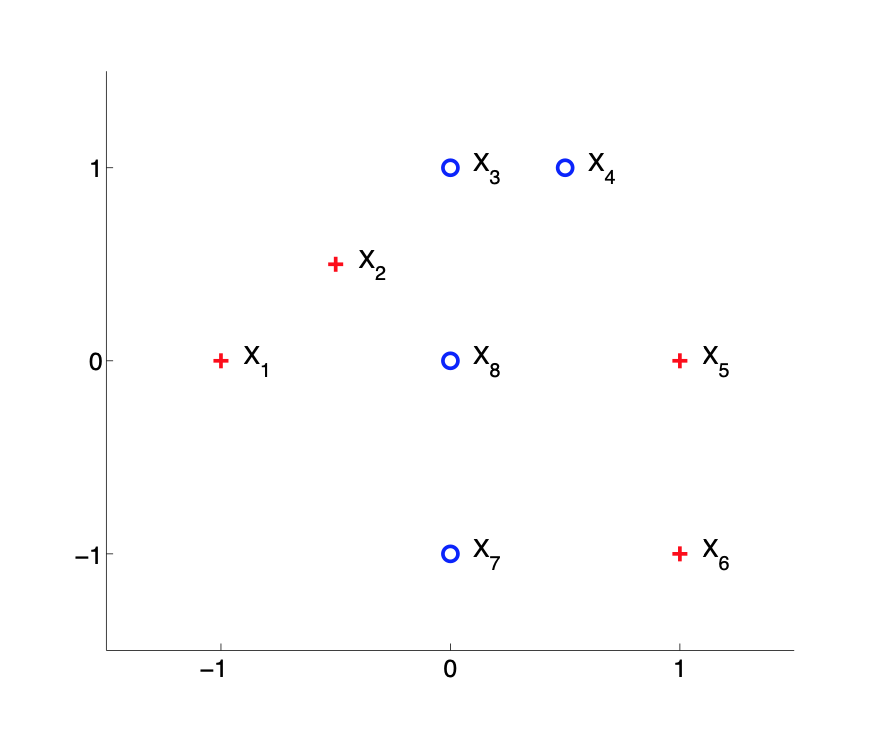
\includegraphics[width = .6\textwidth]{hw}
\end{center}
\caption{ A small dataset, for binary classification with AdaBoost.}
\end{figure}


\begin{table}
\begin{center}
\caption{Values of AdaBoost parameters at each timestep.}
\vspace{0.1in}
\begin{tabular}{|c|c|c|c|c|c|c|c|c|c|c|c|}\hline
t & $\epsilon_t$ & $\alpha_t$ & $Z_t$ & $D_t(1)$ & $D_t(2)$ & $D_t(3)$ & $D_t(4)$ & $D_t(5)$ & $D_t(6)$ & $D_t(7)$ & $D_t(8)$ \\\hline
1 & & & & & & & & & & & \\
2 & & & & & & & & & & &\\
3 & & & & & & & & & & & \\\hline
\end{tabular}
\end{center}
\end{table}

%\item{Boosting algorithms [30 points]}
%
%In this problem, we test your understanding of AdaBoost algorithm. The figure shows a dataset of 8 points, equally divided among the two classes (positive and negative). The figure also shows a particular choice of decision stump $h_1$ picked by Adaboost in the first iteration. 
%
%\begin{figure}[h]%{0.5\textwidth}
%  \begin{center}
%    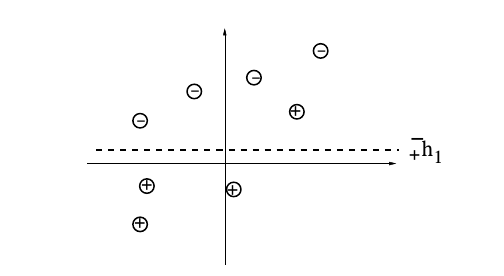
\includegraphics[width=0.7\textwidth]{adaboost.png}
%  \end{center}
%\end{figure}
%
%%\vspace{1cm}
%
%\begin{enumerate}
%\item[(a)] (10 points) Explain the weights $D_2(i)$ for each sample after the first iteration. You can explain by drawing figures similar to what we have in class. 
%
%%\vspace{4cm}
%
%\item[(b)] (10 points) Calculate the weight $\alpha_1$ assigned to $h_1$ by Adaboost? (Note that initial weights of all the data points are equal, $D_1(i) = 1/8, \forall i$ ). 
%%log sqrt(7)%
%%\vspace{3cm}
%
%%\item[(b)] \textbf{[True/False]} AdaBoost will eventually reach zero training error, regardless of the type of weak classifier it uses, provided enough weak classifiers have been combined. }
%% False , Not if the data in the training set cannot be separated by a linear comb bination of the specific type of weak classifiers we are using.%
%
%%\vspace{3cm}
%
%\item[(c)] \textbf{[True/False]} (5 points) The votes $\alpha_i$ assigned to weak classifiers in boosting generally goes down as the algorithm proceeds, because the weighted training error of the weak classifiers tend tends to go up.
%
%% Answer: True In the course of boosting iterations the weak classifiers are forced to try to classify more difficult examples. The weights will increase for examples that are repeatedly misclassified by the weak component classifiers. The weighted training error of the components therefore tends to go up and, as a result, their votes go down.
%%\vspace{2cm}
%
%\item[(d)] \textbf{[True/False]} (5 points) The votes $\alpha$ assigned to the classifiers assembled by Adaboost are always non-negative. 
% Answer: True As defined in class, AdaBoost will choose classifiers with training error above 1/2. %This will ensure that $\log 2 (1+ \epsilon/\epsilon)$, and therefore the vote, is positive. 
% Note that if the classifier does worse than 1/2 we can always assign the sign of its predictions and therefore get a classifier that does slightly better than 1/2. %The vote assigned to the classifier would be non-negative.
%
%\end{enumerate}

\clearpage

\item{\bf Random forest for email spam classifier} (25 points)

Your task for this question is to use random forest to build a spam classifier using the UCR email spma dataset \url{https://archive.ics.uci.edu/ml/datasets/Spambase} came from the postmaster and individuals who had filed spam. The collection of non-spam e-mails came from filed work and personal e-mails, and hence the word \textsf{'george'} and the area code \textsf{'650'} are indicators of non-spam. These are useful when constructing a personalized spam filter. 

%One would either have to blind such non-spam indicators or get a very wide collection of non-spam to generate a general purpose spam filter. Load the data. %
You will see there are total of 4601 instances, and 57 features. 

\begin{enumerate}

\item (5 points) How many instances of spam versus regular emails are there in the data? How many data points there are? How many features there are?

Note: there may be some missing values, you can just fill in zero.

\item (10 points) Build a classification tree model (also known as the CART model). In our answer, you should report the tree models fitted similar to what is shown in the ``Random forest'' lecture, Page 16, the tree plot.

\item (10 points)
Also build a random forrest model. 

Now partition the data to use the first 80\% for training and the remaining 20\% for testing. Your task is to compare and report the AUC  for your classification tree and random forest models on testing data, respectively. To report your results, please try different tree sizes. Plot the curve of AUC versus Tree Size, similar to Page 15 of the Lecture Slides on ``Random Forest''. 


{\it Background information:} In classification problem, we use AUC (Area Under The Curve) as a performance measure. It is one of the most important evaluation metrics for checking any classification model?s performance. ROC (Receiver Operating Characteristics) curve measures classification accuracy at various thresholds settings. AUC measures the total area under the ROC curve. Higher the AUC, better the model is at distinguishing the two classes. If you want to read a bit more about AUC curve, check out this link \url{https://towardsdatascience.com/understanding-auc-roc-curve-68b2303cc9c5} 
\end{enumerate}

\clearpage

\item{\bf Nonlinear regression and cross-validation} (25 points)
 

The coefficient of thermal expansion $y$ changes with temperature $x$. An experiment to relate $y$ to $x$ was done. Temperature was measured in degrees Kelvin. (The Kelvin temperature is the Celsius temperature plus 273.15). The raw data file is \textsf{copper-new.txt}.

\begin{figure}[h!]
\begin{center}
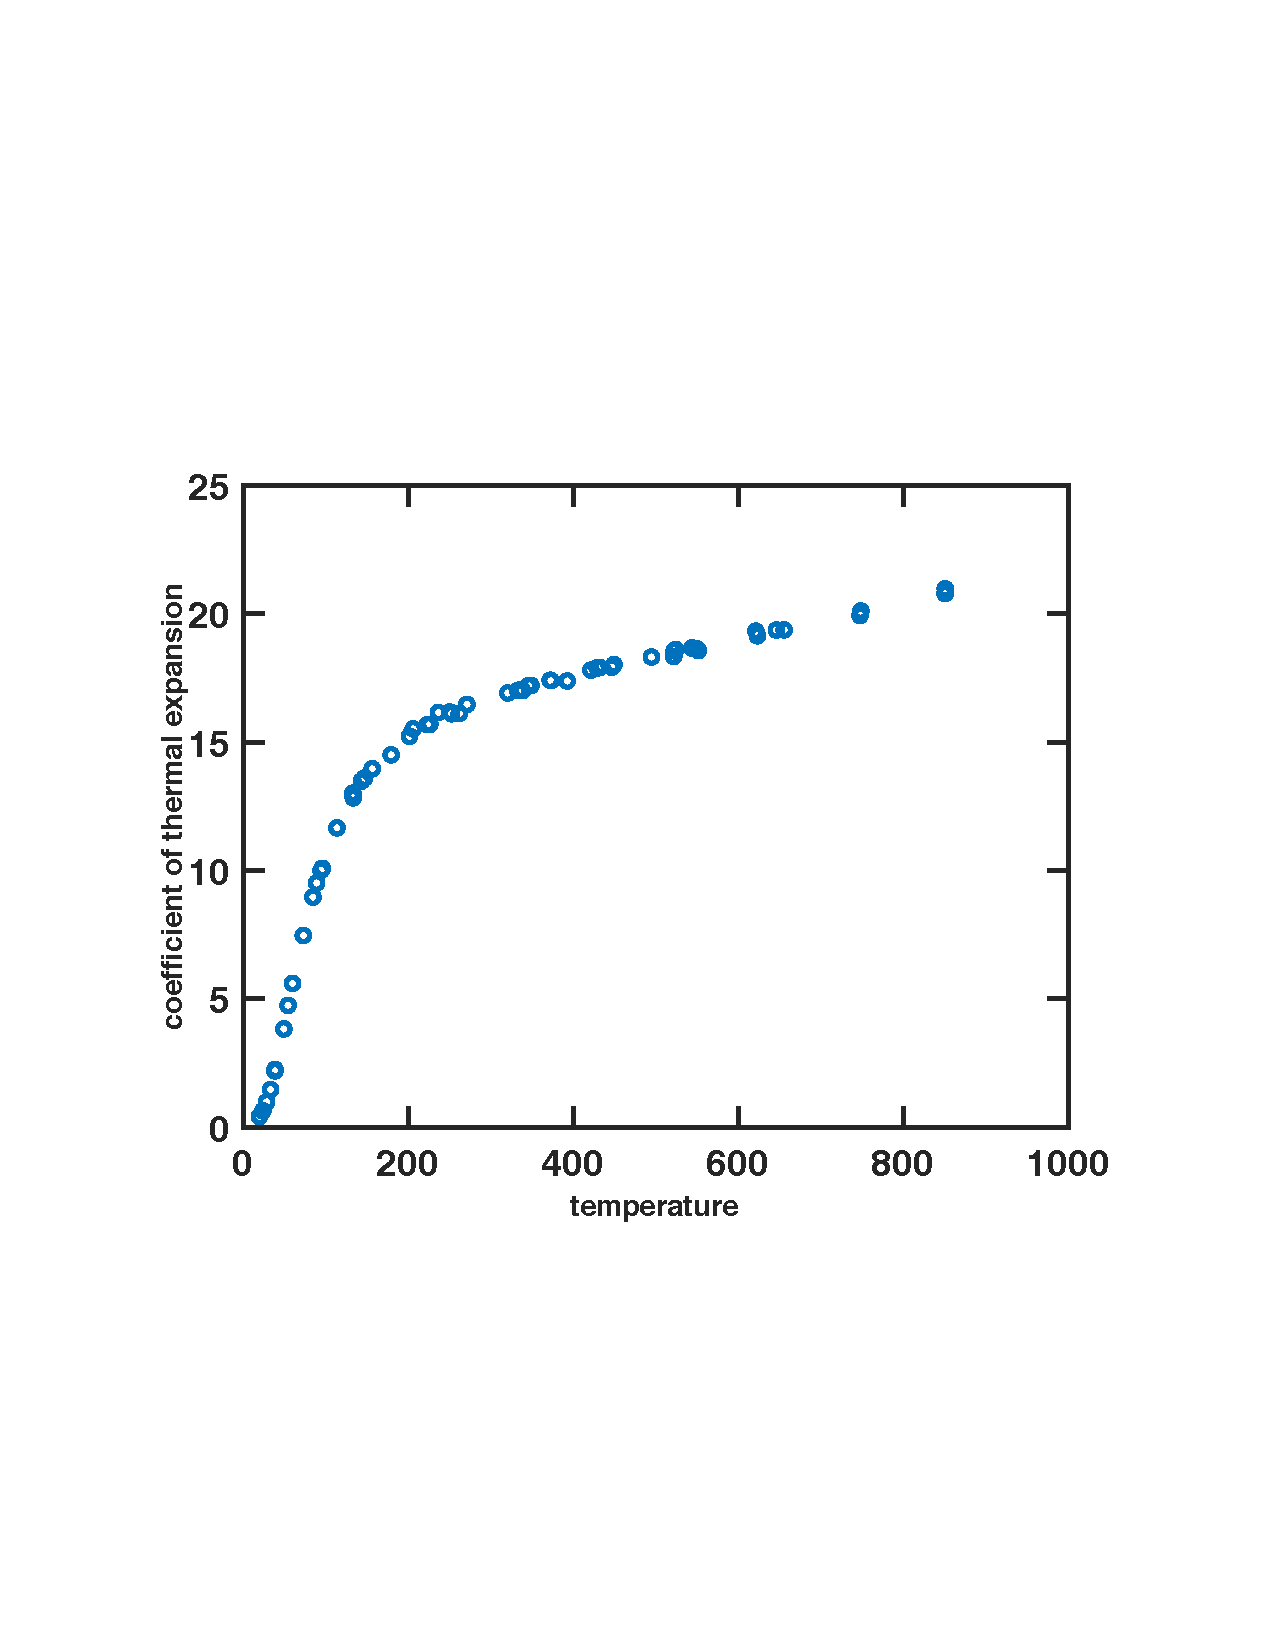
\includegraphics[width = 0.6\textwidth]{t_c}
\end{center}
\end{figure}

\begin{enumerate}

\item (5 points) Perform linear regression on the data. Report the fitted model and the fitting error.
\item (5 points) Perform nonlinear regression with polynomial regression functions up to degree $n = 4$ and use ridge regression (see Lecture Slides for ``Bias-Variance Tradeoff''). Write down your formulation and strategy for doing this, the form of the ridge regression. 
\item (10 points) Use $5$ fold cross validation to select the optimal regularization parameter $\lambda$. Plot the cross validation curve and report the optimal $\lambda$.
\item (5 points) Predict the coefficient at 400 degree Kelvin using both models. Comment on how would you compare the accuracy of predictions. 
\end{enumerate}


\clearpage

\item{\bf Regression, bias-variance tradeoff} (25 points)


Consider a dataset with $n$ data points $(x_i, y_i)$, $x_i \in \mathbb R^p$, drawn from the following linear model:
\[
y = x^T {\beta^*} + \epsilon,
\]
where $\epsilon$ is a Gaussian noise and the star sign is used to differentiate the true parameter from the estimators that will be introduced later. Consider the regularized linear regression as follows:
\[
\hat \beta(\lambda) 
= \arg\min_{\beta}
\left\{
\frac 1 n \sum_{i=1}^n (y_i -x_i^T \beta)^2 + \lambda \|\beta\|_2^2
\right\},
\]
where $\lambda \geq 0$ is the regularized parameter. Let $X\in \mathbb R^{n\times p}$ denote the matrix obtained by stacking $x_i^T$ in each row. 
\begin{enumerate}
\item (10 points) Find the closed form solution for $\hat \beta(\lambda)$ and its distribution.
\item (5 points) Calculate the bias  $\mathbb E[x^T {\hat \beta}(\lambda)] - x^T {\beta^*}$ as a function of $\lambda$ and some fixed test point $x$.
\item (5 points) Calculate the variance term $\mathbb E\left[\left(x^T {\hat \beta}(\lambda) - \mathbb E[x^T {\hat \beta}(\lambda)] \right)^2\right]$.
\item (5 points) Use the results from parts (b) and (c) and the bias-variance decomposition to analyze the impact of $\lambda$ in the squared error. Specifically, which term dominates when $\lambda$ is small, and large, respectively?
\end{enumerate}


(Hint.) Properties of an affine transformation of a Gaussian random variable will be useful throughout this problem.

\end{enumerate}


\end{document}
